\documentclass[15pt, mathserif]{beamer}

\usepackage[french]{babel}
\usepackage[T1]{fontenc}
\usepackage[utf8]{inputenc}
%\usepackage{esvect}
\usepackage{bm}
\usepackage{eurosym}
\usepackage{tikz}
\usepackage{pgf,tikz,pgfplots}
\pgfplotsset{compat=1.15}
\usepackage{mathrsfs}
\usetikzlibrary{arrows}
\usetikzlibrary{arrows.meta}

\usetikzlibrary{mindmap}
\usepackage{multicol}
\usepackage[tikz]{bclogo}
\usepackage{tkz-tab}
\usepackage{amsmath, tabu}
\usepackage{esvect} %\vv{AB} pour le vecteur AB

\DeclareMathOperator{\e}{e}

%% Tableau

\usepackage{makecell}
\setcellgapes{1pt}
\makegapedcells
\newcolumntype{R}[1]{>{\raggedleft\arraybackslash }b{#1}}
\newcolumntype{L}[1]{>{\raggedright\arraybackslash }b{#1}}
\newcolumntype{C}[1]{>{\centering\arraybackslash }b{#1}}


%pour avoir des parenthèses rondes dans le package fourier
\DeclareSymbolFont{cmoperators}   {OT1}{cmr} {m}{n}
\DeclareSymbolFont{cmlargesymbols}{OMX}{cmex}{m}{n}

\usefonttheme{professionalfonts} %permet d'enlever un bug avec fourier
\usepackage{fourier}
\DeclareMathDelimiter{(}{\mathopen} {cmoperators}{"28}{cmlargesymbols}{"00}
\DeclareMathDelimiter{)}{\mathclose}{cmoperators}{"29}{cmlargesymbols}{"01}

%Graphiques 

\usepackage{pgf,tikz,pgfplots}
\pgfplotsset{compat=1.15}
\usepackage{mathrsfs}
\usetikzlibrary{arrows}
\usetikzlibrary{mindmap}

%ensembles de nbres

\newcommand{\R}{\mathbb{R}}			%permet d'écrire le R "ensemble des réels"'
\newcommand{\N}{\mathbb{N}}			%permet d'écrire le N "ensemble des entiers naturels"
\newcommand{\Z}{\mathbb{Z}}			%permet d'écrire le Z "ensemble des entiers relatifs"
\newcommand{\Prem}{\mathbb{P}}	%permet d'écrire le P "ensemble des nombres premiers" (qui n'a pas marché avec le \P car il existe déjà)
\newcommand{\D}{\mathbb{D}}
\newcommand{\Df}{\mathcal{D}_f}
\newcommand{\Cf}{\mathcal{C}_f}

\newcommand{\Q}{\mathbb{Q}}


\newcommand{\st}[1]{$(#1_n)_{n \in \N}$}

\usetheme{Madrid}
\useoutertheme{miniframes} % Alternatively: miniframes, infolines, split
\useinnertheme{circles}
\definecolor{UBCblue}{rgb}{0.1, 0.25, 0.4} % UBC Blue (primary)
\definecolor{bordeaux}{RGB}{128,0,0}
\usecolortheme[named=UBCblue]{structure}

\usepackage{color} % J'aime bien définir mes couleurs
\definecolor{propcolor}{rgb}{0, 0.5, 1}
\definecolor{thcolor}{rgb}{0.6, 0.07, 0.07}
\colorlet{louis}{blue!70!green!60!white}
\colorlet{sakura}{pink!40!red}

\title{Activités Mentales}
\date{24 Août 2023}

\newcommand{\vco}[2]{\begin{pmatrix} #1 \\ #2 \end{pmatrix}} %Coordonnées de vecteur
\newenvironment{eq}{\begin{cases}\begin{tabu}{ccccc}}{\end{tabu}\end{cases}}
\newenvironment{eql}{\begin{cases}\begin{tabu}{cccccl}}{\end{tabu}\end{cases}}
\newenvironment{eqrl}{\begin{cases}\begin{tabu}{rl}}{\end{tabu}\end{cases}}

\newenvironment{Eq}{\begin{center}\begin{tabular}{rrcl}}{\end{tabular}\end{center}}
\newcommand{\ligneq}[2]{$\Longleftrightarrow$ & $#1$ & $=$ & $#2$ \\}
\newcommand{\Ligneq}[2]{ & $#1$ & $=$ & $#2$ \\}

\newenvironment{RPN}{\begin{center}\begin{tabular}{rrclcrcl}}{\end{tabular}\end{center}}
\newcommand{\Lignerpn}[4]{ & $#1$ & $=$ & $#2$ & ou & $#3$ & $=$ & $#4$ \\}
\newcommand{\lignerpn}[4]{$\Longleftrightarrow$ & $#1$ & $=$ & $#2$ & ou & $#3$ & $=$ & $#4$ \\}

\newenvironment{TRPN}{\begin{center}\begin{tabular}{rrclcrclcrcl}}{\end{tabular}\end{center}}
\newcommand{\Lignetrpn}[6]{ & $#1$ & $=$ & $#2$ & ou & $#3$ & $=$ & $#4$ & ou & $#5$ & $=$ & $#6$ \\}
\newcommand{\lignetrpn}[6]{$\Longleftrightarrow$ & $#1$ & $=$ & $#2$ & ou & $#3$ & $=$ & $#4$ & ou & $#5$ & $=$ & $#6$ \\}
\begin{document}

\begin{frame}
    \titlepage
\end{frame}

\begin{frame} 
	\frametitle{Question 1}
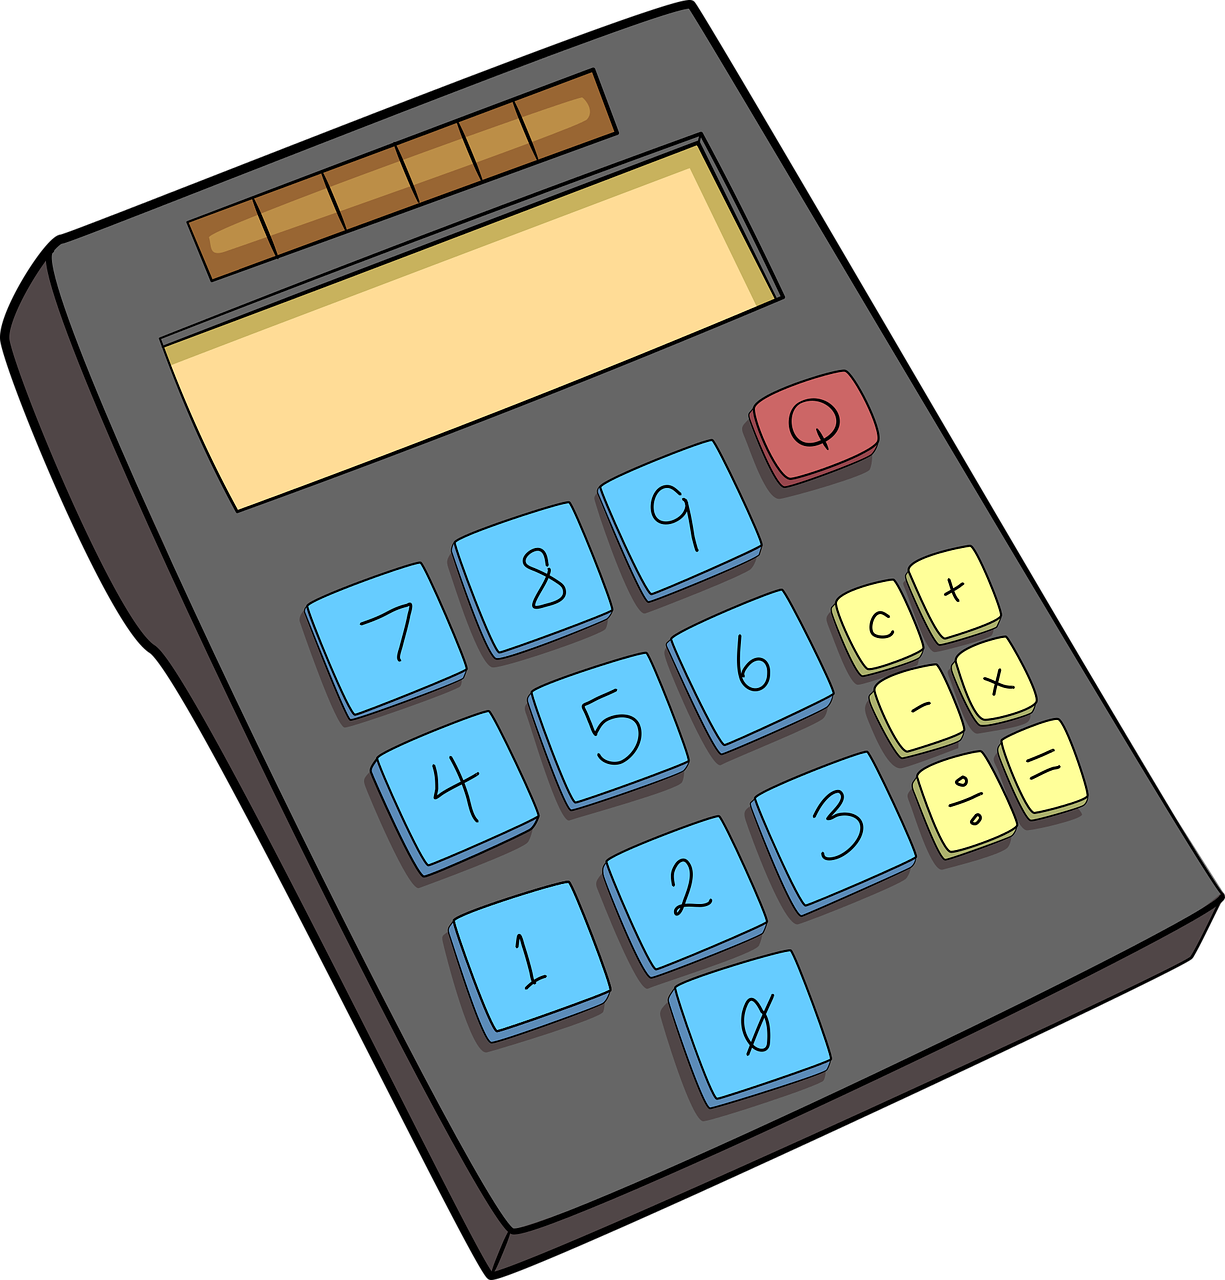
\includegraphics[scale=0.01]{calculatrice}Un article était vendu 28.19\euro ~ est vendu 11.96\euro ~ après réduction. Quel est le pourcentage appliqué pour la réduction? \end{frame}


\begin{frame} 
	\frametitle{Question 2}
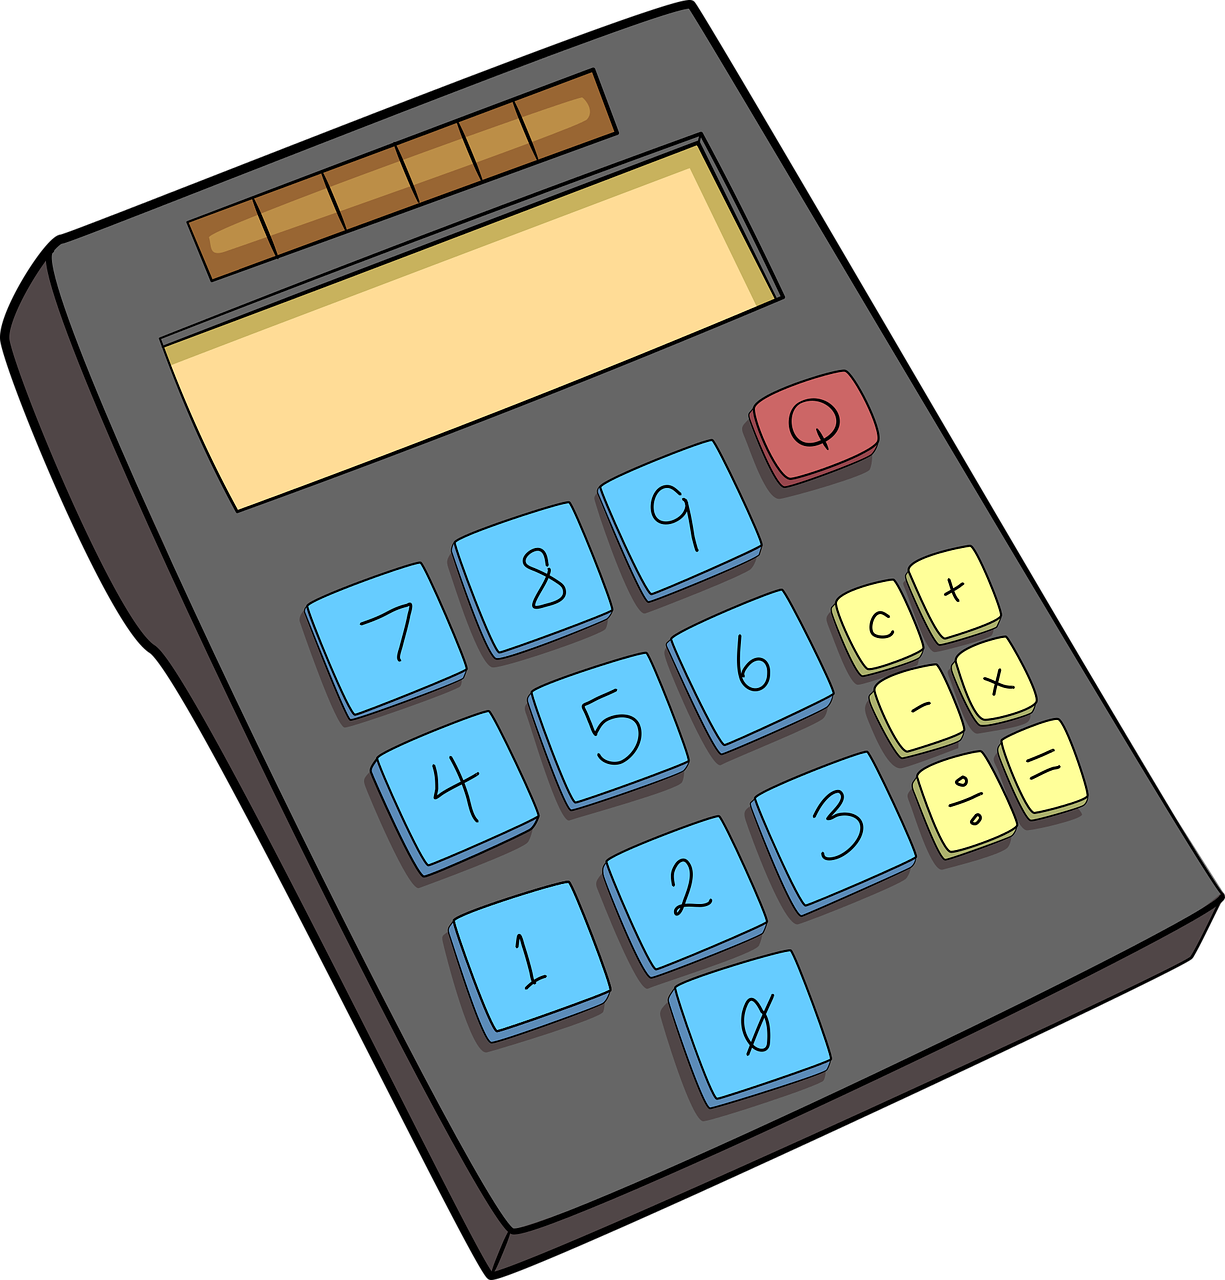
\includegraphics[scale=0.01]{calculatrice}Ci-dessous sont résumés les tarifs d'un parking en 2016 et en 2018. 
 \begin{center} 
 \begin{tabular}{|C{3cm}|c|c|} 
 \hline 
 Type de véhicule (pour 24h) & 2016 & 2018 \\ 
 \hline 
 Véhicule individuel & 11.01& 11.15\\ 
 \hline 
 Camping-car & 16.01& 16.15\\ 
 \hline 
 Moto & 5.5& 5.58\\ 
 \hline 
 \end{tabular} 
\end{center} 
  Quelle est l'évolution du prix du parking en \% pour les Véhicules individuels ? \end{frame}


\begin{frame} 
	\frametitle{Question 3}
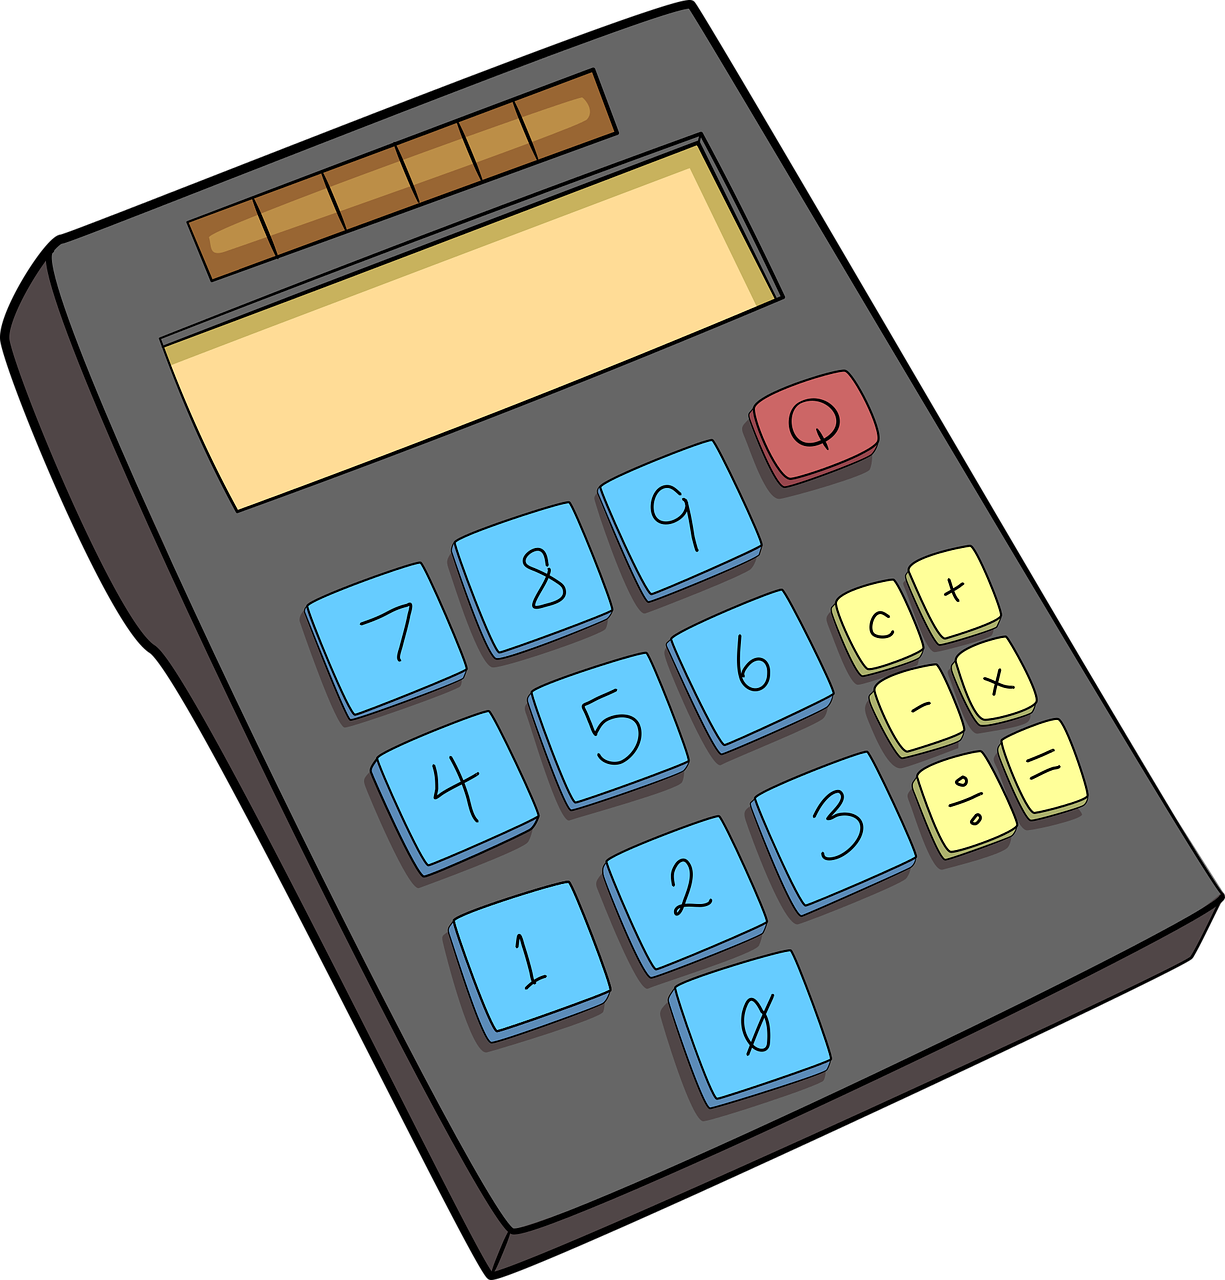
\includegraphics[scale=0.01]{calculatrice}Un article était vendu 22.19\euro ~ est vendu 20.31\euro ~ après réduction. Quel est le pourcentage appliqué pour la réduction? \end{frame}


\begin{frame} 
	\frametitle{Question 4}
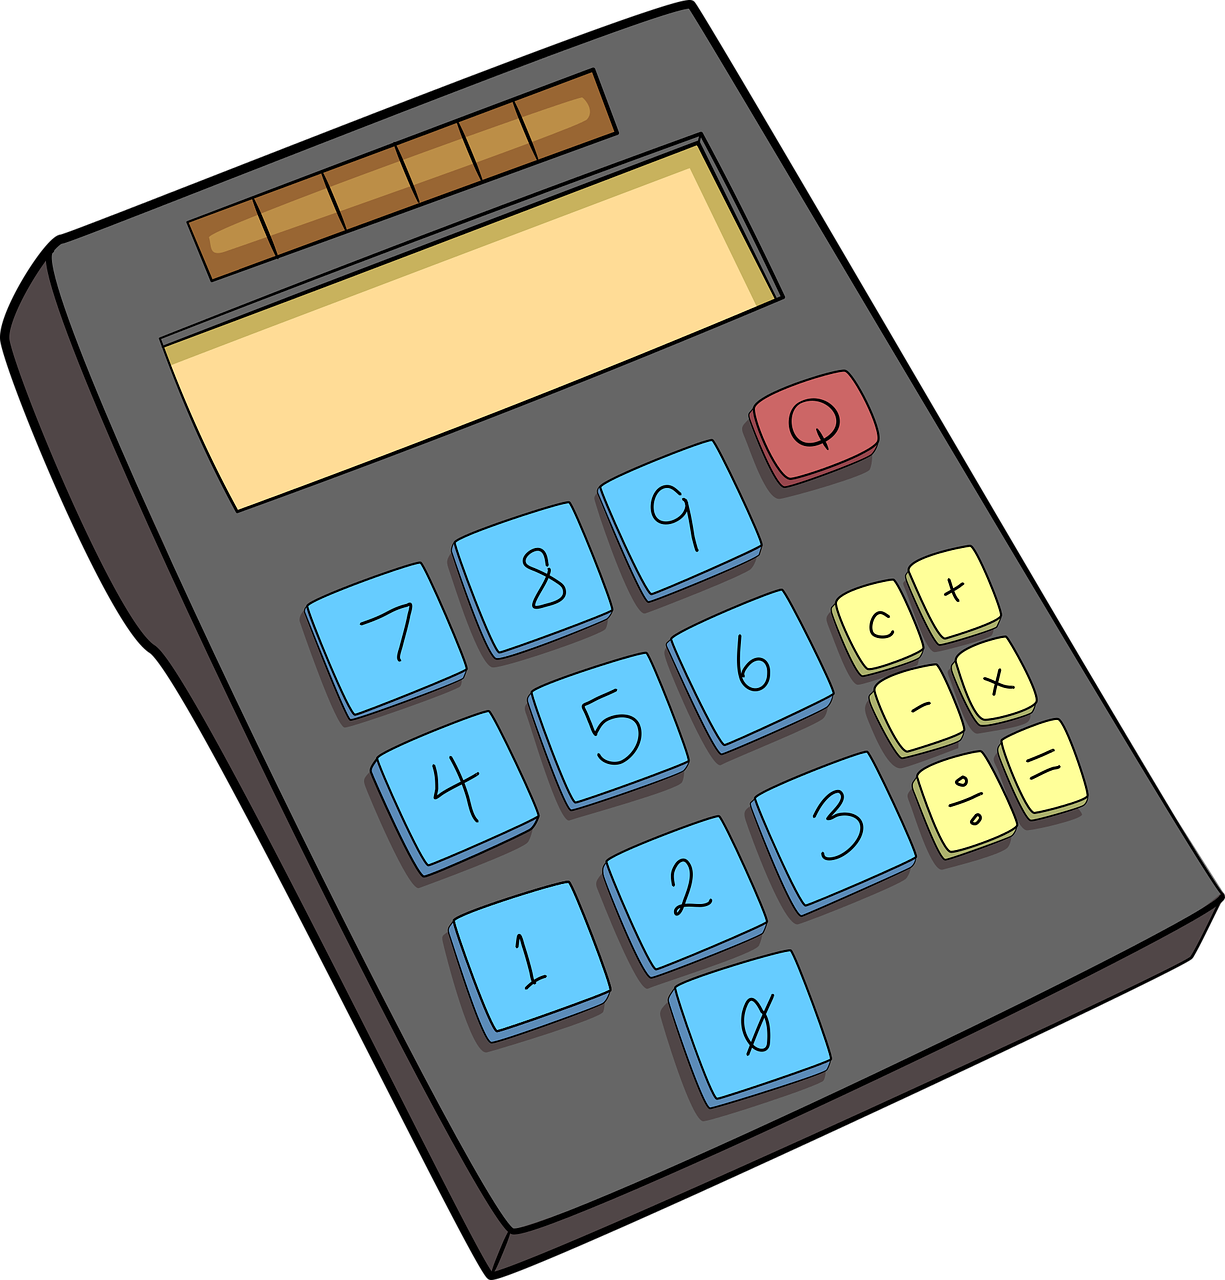
\includegraphics[scale=0.01]{calculatrice}Ci-dessous sont résumés les tarifs d'un parking en 2016 et en 2018. 
 \begin{center} 
 \begin{tabular}{|C{3cm}|c|c|} 
 \hline 
 Type de véhicule (pour 24h) & 2016 & 2018 \\ 
 \hline 
 Véhicule individuel & 10.24& 11.18\\ 
 \hline 
 Camping-car & 15.24& 16.18\\ 
 \hline 
 Moto & 5.12& 5.59\\ 
 \hline 
 \end{tabular} 
\end{center} 
  Quelle est l'évolution du prix du parking en \% pour les Camping-cars ?\end{frame}


\begin{frame} 
	\frametitle{Question 5}
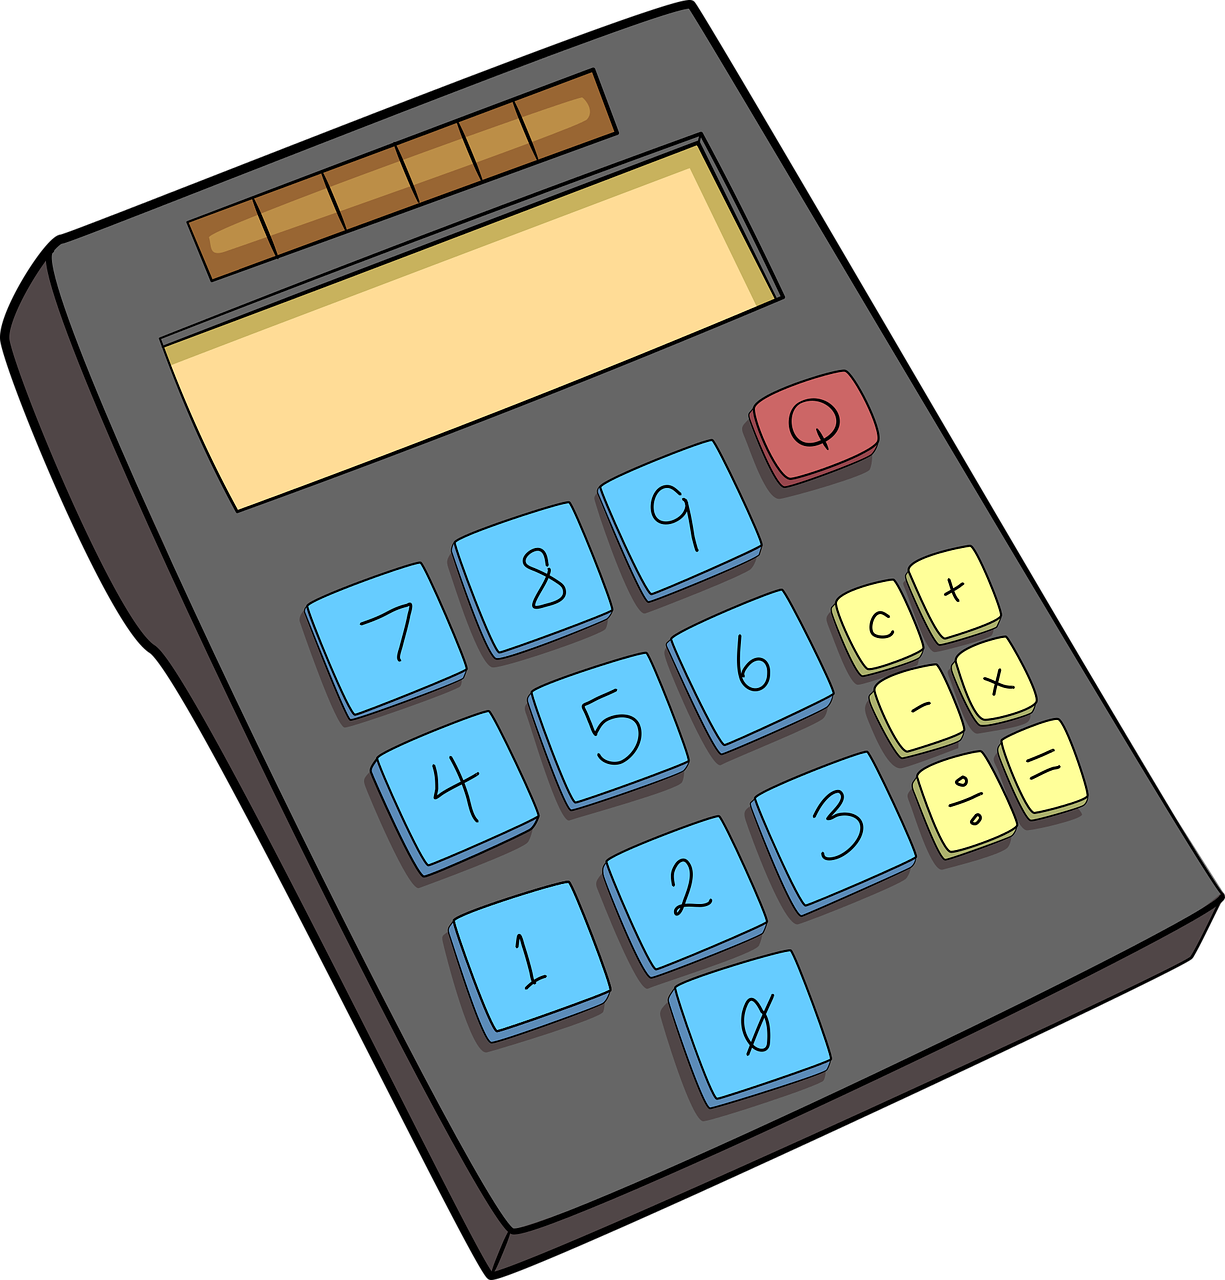
\includegraphics[scale=0.01]{calculatrice}Un article était vendu 37.13\euro ~ est vendu 19.97\euro ~ après réduction. Quel est le pourcentage appliqué pour la réduction? \end{frame}


\begin{frame}
\vspace{-10mm}
	\frametitle{Correction 1}
Un article était vendu 28.19\euro ~ est vendu 11.96\euro ~ après réduction. Quel est le pourcentage appliqué pour la réduction? \\ Ici le prix a changé dans le temps donc on doit calculer un taux d'évolution. On doit donc appliquer la formule $$\dfrac{V_f-V_i}{V_i}$$ avec $V_i =28.19$ et $V_f=11.96$. On a alors en remplaçant dans la formule $$\dfrac{11.96-28.19}{28.19}= \dfrac{-16.23}{28.19}=-0.5757$$ La réduction appliquée est donc de 57.57\%.\end{frame}


\begin{frame}
\vspace{-10mm}
	\frametitle{Correction 2}
 
 \begin{center} 
 \begin{tabular}{|C{3cm}|c|c|} 
 \hline 
 {\small Type de véhicule} & {\small 2016} & {\small 2018} \\ 
 \hline 
 {\small Véhicule individuel} & 11.01& 11.15\\ 
 \hline 
 {\small Camping-car } & 16.01& 16.15\\ 
 \hline 
 {\small Moto } & 5.5& 5.58\\ 
 \hline 
 \end{tabular} 
\end{center} 
  {\small Quelle est l'évolution du prix du parking en \% pour les Véhicules individuels ? \\ Ici on a une évolution du prix en fonction du temps. On doit donc appliquer la formule} $$\dfrac{V_f-V_i}{V_i}$$ avec $V_i =11.01$ et $V_f=11.15$. {\small On a alors en remplaçant dans la formule} $$\dfrac{11.15-11.01}{11.01}= \dfrac{0.14}{11.01} = 0.01$$ {\small Le prix a donc augmenté de  1.0\% } \end{frame}


\begin{frame}
\vspace{-10mm}
	\frametitle{Correction 3}
Un article était vendu 22.19\euro ~ est vendu 20.31\euro ~ après réduction. Quel est le pourcentage appliqué pour la réduction? \\ Ici le prix a changé dans le temps donc on doit calculer un taux d'évolution. On doit donc appliquer la formule $$\dfrac{V_f-V_i}{V_i}$$ avec $V_i =22.19$ et $V_f=20.31$. On a alors en remplaçant dans la formule $$\dfrac{20.31-22.19}{22.19}= \dfrac{-1.88}{22.19}=-0.0847$$ La réduction appliquée est donc de 8.47\%.\end{frame}


\begin{frame}
\vspace{-10mm}
	\frametitle{Correction 4}
 
 \begin{center} 
 \begin{tabular}{|C{3cm}|c|c|} 
 \hline 
 {\small Type de véhicule} & {\small 2016} & {\small 2018} \\ 
 \hline 
 {\small Véhicule individuel} & 10.24& 11.18\\ 
 \hline 
 {\small Camping-car } & 15.24& 16.18\\ 
 \hline 
 {\small Moto } & 5.12& 5.59\\ 
 \hline 
 \end{tabular} 
\end{center} 
  {\small Quelle est l'évolution du prix du parking en \% pour les Camping-cars ?\\ Ici on a une évolution du prix en fonction du temps. On doit donc appliquer la formule} $$\dfrac{V_f-V_i}{V_i}$$ avec $V_i =15.24$ et $V_f=16.18$. On a alors en remplaçant dans la formule $$\dfrac{16.18-15.24}{15.24}= \dfrac{0.94}{15.24} = 0.0617$$ {\small Le prix a donc augmenté de  6.17\% } \end{frame}


\begin{frame}
\vspace{-10mm}
	\frametitle{Correction 5}
Un article était vendu 37.13\euro ~ est vendu 19.97\euro ~ après réduction. Quel est le pourcentage appliqué pour la réduction? \\ Ici le prix a changé dans le temps donc on doit calculer un taux d'évolution. On doit donc appliquer la formule $$\dfrac{V_f-V_i}{V_i}$$ avec $V_i =37.13$ et $V_f=19.97$. On a alors en remplaçant dans la formule $$\dfrac{19.97-37.13}{37.13}= \dfrac{-17.16}{37.13}=-0.4622$$ La réduction appliquée est donc de 46.22\%.\end{frame}




\end{document}